\section{Zustandsbasierter Test}


\begin{tcolorbox}[title=Zustandsbasierter Test]
    Wenn eine Methode einer Klasse bei unterschiedlichen Feldern ein anderes Verhalten zeigt, ist das Verhalten von dem \textbf{inneren Zustand abhängig}.\\
    Da sich dies auf Testgegenstände auswirkt, muss das unterschiedliche Verhalten in den verschiedenen Zuständen getestet werden.\\

    \noindent
    In einfachen Fällen können die benötigten Testfälle ohne Formalismus erraten werden; für kompliziertere Fälle wird ein systematisches Vorgehen benötigt, damit nichts übersehen wird.\\
    Hierzu wird zunächst ein \textbf{UML-Zustandsdiagramm} der Zustände und ihrer Zustandsübergänge erstellt, woraufhin dann eine Zustandsübergangstabelle  erstellt wird, aus der alle Zustände und Ereignisse mit ihren Folgezuständen abgelesen werden können.
\end{tcolorbox}


\begin{table}[]
    \centering
    \setlength{\tabcolsep}{0.5em}
    \def\arraystretch{1.5}
    \begin{tabular}{|l|c|l|c|}
        \hline
        & \textbf{empty}                                                                     & \multicolumn{1}{c|}{\textbf{filled}}                                                                          & \textbf{full}                                                                     \\ \hline
        \code{push()} & filled                                                                             & \begin{tabular}[c]{@{}l@{}}{[}size\textless{}maxsize-1{]}: filled\\ {[}size = maxsize-1{]}: full\end{tabular} & \begin{tabular}[c]{@{}c@{}}full\\ \textless{}Exception\textgreater{}\end{tabular} \\ \hline
        \code{pop()}  & \begin{tabular}[c]{@{}c@{}}empty\\ \textless{}Exception\textgreater{}\end{tabular} & \begin{tabular}[c]{@{}l@{}}{[}size>1{]} : filled\\ {[}size=1{]}: empty\end{tabular}                       & filled                                                                            \\ \hline
    \end{tabular}
    \caption{Zustandsübergangstabelle für das Beispiel \textit{Stack}. Die Inhalte der Tabelle sind die Folgezustände; in spitzen Klammern stehen die Ergebnisse bei verbotenen Übergängen. (Quelle: \cite[Tab. 5.1, 48]{Wed09c})}
    \label{tab:popstate-cc}
\end{table}

\vspace{5mm}
\begin{tcolorbox}[colback=red!20,title={Notation für \textit{Event[Guard]}}]
    \textit{Wedemann} verwendet den Doppelpunkt ``:`` als Separator für die Notation \textit{Event[Guard]} (lies: ``das Ereignis wird getriggert, wenn der Guard zu $true$ evaluiert.``) in Abbildung~\ref{fig:popstate-cc}.\\
    Für diese Notation findet sich in \cite[320 f.]{OMG17} kein Hinweis.
\end{tcolorbox}
\vspace{5mm}

\begin{figure}
    \centering
    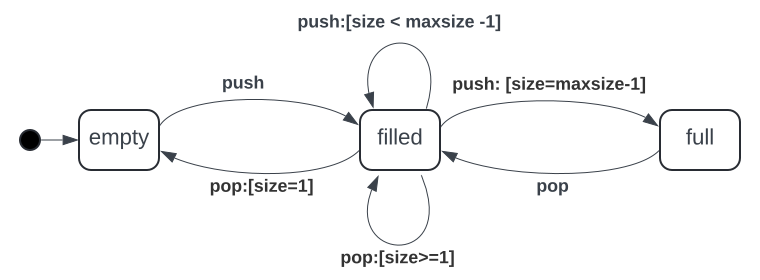
\includegraphics[scale=0.5]{part four/Testende Verfahren/img/popstate}
    \caption{UML-Zustandsdiagramm für Objekte der Klasse \textit{Stack}. (Quelle: in Anlehnung an \cite[Abb. 5.1, 47]{Wed09c})}
    \label{fig:popstate-cc}
\end{figure}